\documentclass[portuguese,noindentfirst]{UASTeX} % or \documentclass[english]{UASTeX}

\title{UAS\TeX: Modelo de Trabalho de Conclusão de Curso do Bacharelado em Sistemas de Informação da UAST} % required

\mainauthor{Maria Souza Santos} % required

\advisor{Estevan Dias Ferreira} % required
\advisorgender{male} % required only for portuguese
\advisorprefix{Dr.} % optional
% \advisorsuffix{, PhD} % optional

\coadvisor{Vitória Carvalho Lima} % optional
\coadvisorgender{female} % only for portuguese
\coadvisorprefix{Dra.} % optional
% \coadvisorsuffix{, PhD} % optional

\date{2023}

\authors{
    \themainauthor\inst{1},
    Luís Rocha Correia\inst{1,2},
    Flávio Rech Wagner\inst{2}, \\
    \thecoadvisor\inst{3}, 
    \theadvisor\inst{1}
}

\address{\uastaddress
\nextinstitute
Centro de Informática (CIn)\\
Universidade Federal de Pernambuco (UFPE)\\
Recife -- PE -- Brasil
\nextinstitute
Escola Politécnica de Pernambuco (POLI)\\
Universidade de Pernambuco (UPE)\\
Recife -- PE -- Brasil\\
} 

\email{
    {\tt\footnotesize\{maria.souza,luis.rocha,estevan.dias\}@ufrpe.br, frw@cin.ufpe.br,} \\
    {\tt\footnotesize vitoria.carvalho@poli.br}
} % you must enter your information here
\begin{acronym}[ACRONYM] 
\acroplural{AP}[APs]{Access Points}
\acro{ABNT}[ABNT]{Associação Brasileira de Normas Técnicas}
\acro{CAPES}[CAPES]{Coordenação de Aperfeiçoamento de Pessoal de Nível Superior}
\acro{NDN}[NDN]{Named Data Networking}
\acro{SBC}[SBC]{Sociedade Brasileira de Computação}
\end{acronym} % define your acronyms here

\begin{document} 

\begin{abstract} % required
        This work presents the main features of UAS\TeX~for writing undergraduate dissertations. UAS\TeX~is a template based on the SBC scientific paper standard. For papers in english, you should add just an abstract while for the papers in portuguese, we also ask for an abstract in portuguese. In both cases, abstracts should not have more than 10 lines and must be in the first page of the paper.
\end{abstract}

\begin{resumo} % it works only when the language is portuguese (documentclass option)
        Este trabalho apresenta as principais características do UAST\TeX~para a elaboração dos trabalhos de conclusão de curso. O UAST\TeX~ é um modelo baseado no padrão de artigo científico da SBC. Artigos em inglês deverão apresentar apenas abstract. É solicitada a escrita de resumo e abstract apenas para os artigos escritos em português. Nos dois casos, o autor deve tomar cuidado para que o resumo (e o abstract) não ultrapassem 10 linhas cada, sendo que ambos devem estar na primeira página do artigo.
\end{resumo}


\section{Introdução}\label{sec:intro}
Este modelo \LaTeX~de trabalho de conclusão de curso foi criado para facilitar o processo da escrita científica dos alunos do Bacharelado em Sistemas de Informação da UAST--UFRPE. Com este modelo o aluno ficará com maior liberdade para se concentrar no conteúdo do trabalho em si, ao invés da formatação do texto. No primeiro contato com a sintaxe do \LaTeX~é normal ter um estranhamento inicial, afinal é uma tecnologia que muitos iniciantes na escrita científica ainda não estão acostumados. Por isso, é necessário um pouco de esforço inicial para aprender os comandos \LaTeX. Não se preocupe, a curva de aprendizado para os comandos básicos do \LaTeX~é muito rápida. Será muito mais divertido desenvolver seu trabalho de conclusão de curso aqui no \LaTeX, quando comparado com o Microsoft Word\textregistered~(ou similares).

Muitos iniciantes confundem \TeX~\cite{knuth:91} com \LaTeX~\cite{lamport:94}. \TeX~é um sistema de tipografia projetado por Donald Ervin Knuth, professor emérito da Universidade de Stanford, a principal referência da análise de algoritmos e conhecido por ser o ``pai'' da área. \TeX~é muito poderoso, os mais atentos conseguem diferenciar facilmente um trabalho científico desenvolvido com \TeX, de outro com o mesmo modelo, mas escrito no Microsoft Word\textregistered. Apesar de robusta, \TeX~é uma linguagem desajeitada e pouco amigável para os iniciantes. Por causa disso, \LaTeX~foi desenvolvido por Leslie Lamport para facilitar a elaboração de trabalhos acadêmicos. \LaTeX~é um conjunto de macros escritas em \TeX. Fazendo uma analogica com linguagens de programação modernas, diríamos que \TeX~é a linguagem de programação e \LaTeX~é o \emph{framework} para escrita de trabalhos científicos. Além disso, a pronúncia de \TeX~é ``tec'' e de \LaTeX~ é ``leitec''. De forma análoga, pronunciamos UAS\TeX~ como ``uastec''.

\section{Sobre o Modelo UAS\TeX}\label{sec:uastex}

O UAS\TeX~é um modelo baseado no padrão de artigo científico da \ac{SBC}. UAS\TeX~suporta trabalhos escritos tanto em português, quanto em inglês. Qualquer dúvida sobre o modelo, você pode entrar em contato comigo através do endereço {\tt ygor.amaral@ufrpe.br}.

A princípio, você deve configurar o arquivo {\tt settings.tex} para adicionar as informações de metadados do seu trabalho. Não esqueça de definir suas siglas em {\tt acronyms.tex}. Não deixe para definir suas siglas manualmente no texto. O pacote acronym do \LaTeX~irá gerenciar para você quando você usou a sua sigla pela primeira vez. Observe que agora a sigla \ac{SBC} não aparece mais com o seu respectivo significado.

\section{Seções e Parágrafos}\label{sec:about_secpar}

Observe como é simples criar as seções com \LaTeX. Ele cuidará de toda a formatação para você! Por padrão, este modelo está configurado para o primeiro parágrafo não ser indentado. Esse é o padrão em qualquer lugar desenvolvido do mundo. Se por acaso algum fanático das normas da \ac{ABNT} solicitar a indentação na primeira linha, respire fundo e modifique a primeira linha deste documento. Use a opção {\tt indentfirst} ao invés de {\tt noindentfirst} no {\tt documentclass}.

\subsection{Subseção}

Você também pode criar subseções.

\subsubsection{Subsubseção}
Esse é o último nível de subseção disponível em UAS\TeX, se você acha que precisa de mais níveis de subseções, recomendo organizar melhor o seu trabalho. =)

\section{Figuras, Tabelas e Legendas}\label{sec:figs_tables_caps}
Como todo modelo de trabalho científico, UAS\TeX~também oferece suporte a Figuras, Tabelas e suas respectivas legendas.

Evite ao máximo inserir imagens no formato jpg ou png. Utilize jpg apenas para fotos. Hoje em dia poucas pessoas imprimem os artigos científicos em papel. O mais habitual é ler esses trabalhos em dispositivos eletrônicos, nos quais podemos aplicar zoom, o quanto desejarmos. O problema de jpg e png é que por serem formatos ``rasterizados'' a qualidade das imagens deteriora rapidamente a cada nível de zoom. Qualquer ferramenta moderna de ilustração, gráficos e diagramas consegue exportar as imagens em formato vetorial. Recomendo exportar suas imagens no formato pdf. Observe como eu incluí as minhas imagens nesse modelo. Aplique a quantidade de zoom que desejar ao observar as Figuras~\ref{fig:network_topology} e~\ref{fig:packet_forwarding}.

Vou aproveitar a Figura~\ref{fig:network_topology} para demonstrar como usar uma sigla no plural. Observe que na Figura~\ref{fig:network_topology} existem três \acp{AP}.

\begin{figure}[ht]
	\centering
	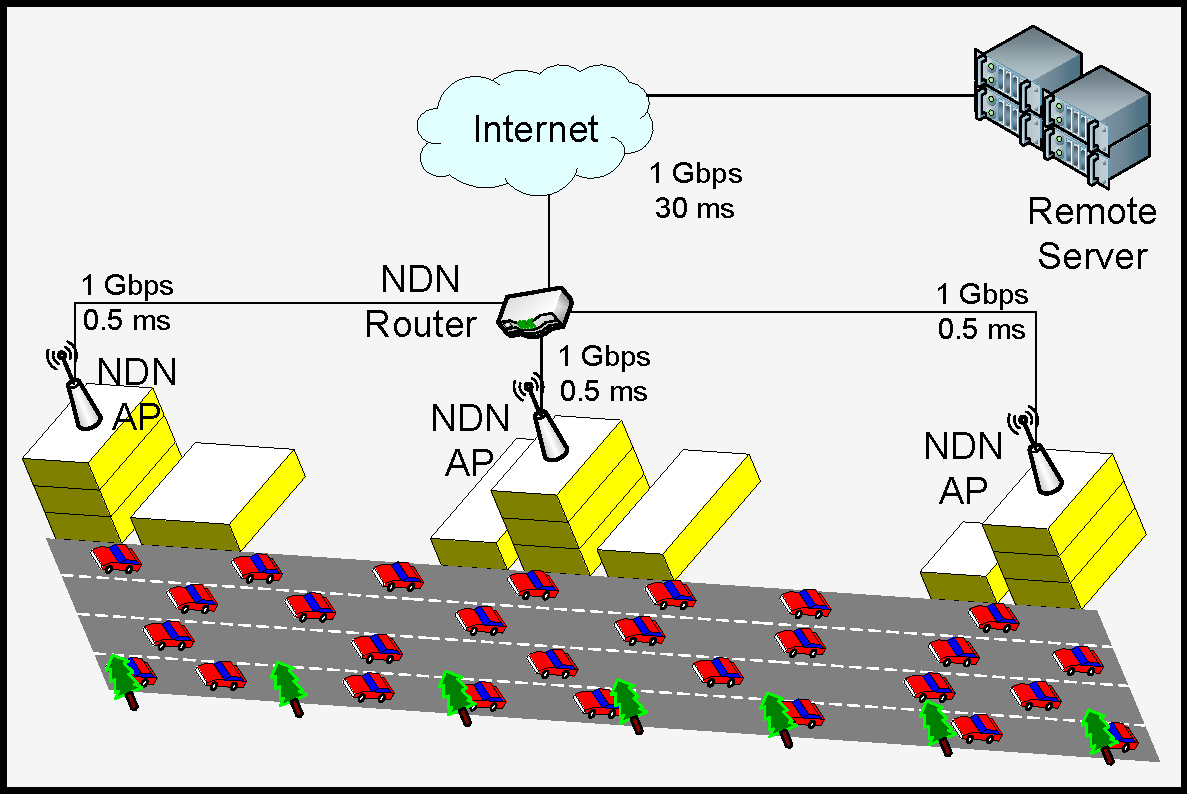
\includegraphics[width=.6\textwidth]{images/illustrations/network_topology}
	\caption{Uma ilustração qualquer, exportada de forma vetorial para pdf.}
	\label{fig:network_topology}
\end{figure}

Vou colocar um pouco mais de texto aqui, apenas para preencher o documento. \lipsum[1-3]

\begin{figure}[ht]
	\centering
	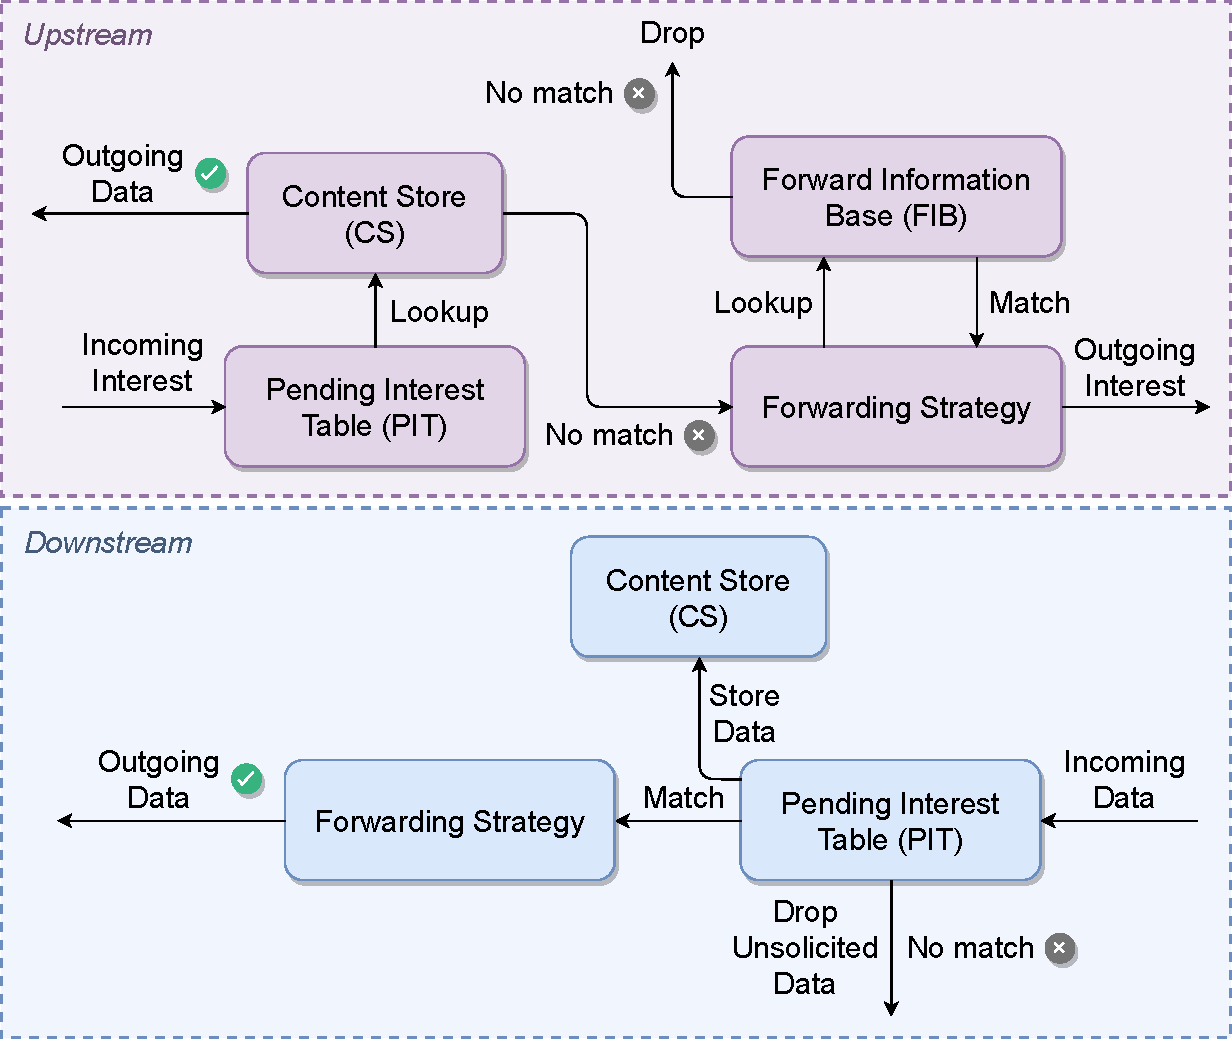
\includegraphics[width=.6\textwidth]{images/illustrations/packet_forwarding}
	\caption{Essa ilustração também é vetorial e possui uma legenda longa que possui mais do que uma linha. Observe nesse caso, que a legenda fica justificada e não mais centralizada.}
	\label{fig:packet_forwarding}
\end{figure}

Diferentemente das Figuras, as legendas das Tabelas ficam no topo. Além disso, a sintaxe das tabelas em \LaTeX~não é das mais amigáveis, mas não se engane, você pode construir qualquer formato de tabela por aqui. A Tabela~\ref{tab:list_evaluated_scenarios} contém alguma informação qualquer.

\begin{table}[htbp]
	\centering
	\caption{Native \ac{NDN} deployment instances}
	\begin{tabular}{cccc}
		\hline Native \ac{NDN} Deployment & Link layer operating mode & Scenarios & Instance\\ 
		\hline
		\hline \multirow{2}{*}{Standard} & \multirow{2}{*}{Broadcast in both directions} & 1 & Standard-1  \\
		\cline{3-4} & & 2 & Standard-2 \\
		\hline \multirow{2}{*}{Up} & \multirow{2}{*}{Unicast upstream only} & 1 & Up-1   \\
		\cline{3-4} & & 2 & Up-2   \\
		\hline \multirow{2}{*}{Down} & \multirow{2}{*}{Unicast downstream only} & 1 & Down-1   \\
		\cline{3-4} & & 2 & Down-2   \\
		\hline \multirow{2}{*}{Proposal} & \multirow{2}{*}{Unicast in both directions} & 1 & Proposal-1   \\
		\cline{3-4} & & 2 & Proposal-2   \\
		\hline
	\end{tabular}
	\label{tab:list_evaluated_scenarios}
\end{table}

\lipsum[1-1]

\subsection{Resultados}\label{sec:results}

Aqui eu vou simplesmente jogar alguns gráficos aleatórios apenas para ilustrar o nosso modelo UAS\TeX. O teste u de mann-whitney pode ser observado no gráfico da Figura~\ref{fig:mw}.

\begin{figure}[ht]
	\centering
	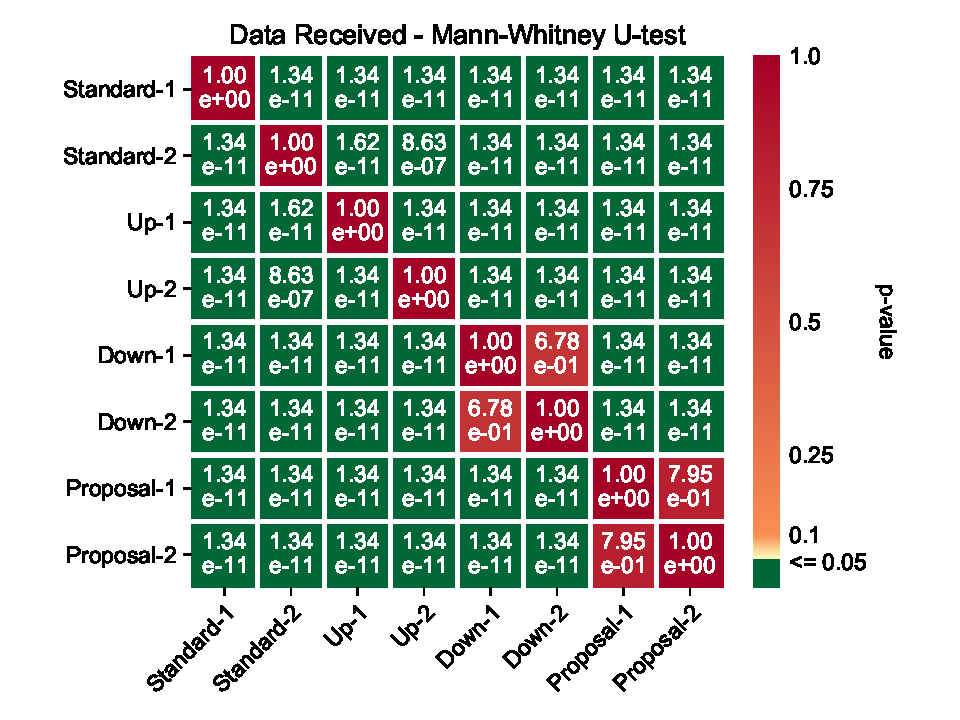
\includegraphics[width=.6\textwidth]{images/charts/mw}
	\caption{Teste U de Mann-Whitney para algum dado qualquer.}
	\label{fig:mw}
\end{figure}

\lipsum[1-1]

\begin{figure}[ht]
	\centering
	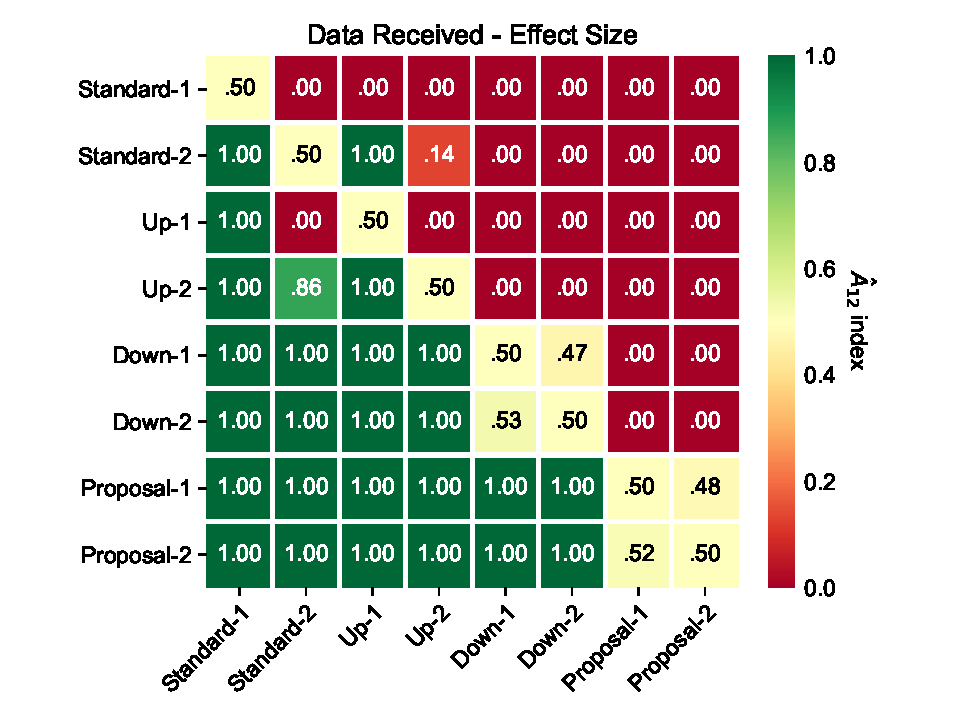
\includegraphics[width=.6\textwidth]{images/charts/vd}
	\caption{Índice $\hat{A}_{12}$ de Vargha e Delaney para algum dado qualquer.}
	\label{fig:vd}
\end{figure}

O índice $\hat{A}_{12}$ de Vargha e Delaney pode ser observado no gráfico da Figura~\ref{fig:vd}.
\lipsum[1-1]

\begin{figure}[ht]
	\centering
	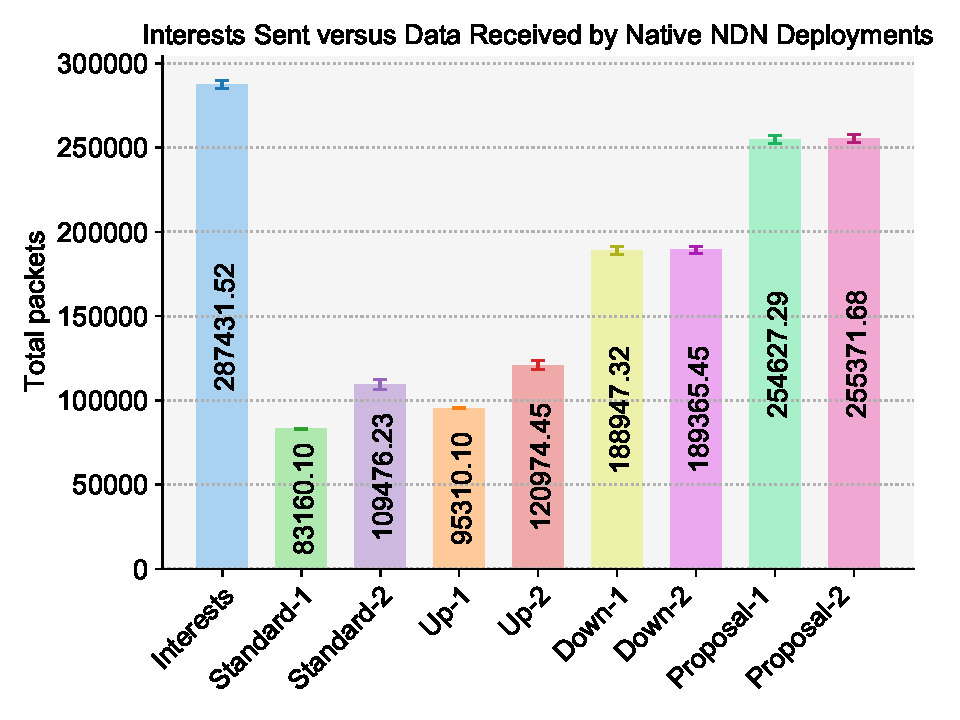
\includegraphics[width=.6\textwidth]{images/charts/bar}
	\caption{Gráfico de barras para algum dado qualquer.}
	\label{fig:bar}
\end{figure}

O gráfico de barras pode ser observado na Figura~\ref{fig:bar}.
\lipsum[1-1]

\section{Gerenciamento das Referências}\label{sec:reference_management}
O UAS\TeX~usa o gerenciador de bibliografia Bib\TeX. O Bib\TeX~é amplamente usado nos trabalhos científicos elaborados com \LaTeX. Existem outros gerenciadores, até mais completos que o Bib\TeX, mas que nunca se tornaram o padrão das principais revistas e congressos científicos na área de computação.

Para adicionar novas referências, acesse o arquivo {\tt references.bib} na pasta {\tt bibliography} e adicione quantas referências for preciso. Elas só aparecerão na seção de referências quando forem citadas através do comando {\tt\textbackslash  cite\{\}}. Como por exemplo:~\cite{knuth:91} e~\cite{lamport:94}.

Para acessar gratuitamente os artigos científicos, você precisará criar sua senha de serviços integrados no sig@ (versão antiga) no endereço {\tt http://www.siga.ufrpe.br}. Depois você poderá acessar o portal dos periódicos da \ac{CAPES} no endereço {\tt http://periodicos.capes.gov.br}. Através do portal da \ac{CAPES}, você poderá ter acesso de forma autenticada ao \emph{Google Scholar}, \emph{Web of Science}, \emph{Scopus}, \emph{IEEE Xplore}, \emph{ACM Digital Library}, \emph{ScienceDirect}, \emph{SpringerLink}, \emph{Wiley Online Library}, entre outros indexadores de artigos científicos relevantes para a computação e áreas afins. Além disso, você poderá acessar gratuitamente os artigos dos eventos da \ac{SBC} sem a necessidade de autenticação pelo portal da \ac{CAPES}, através do endereço {\tt https://sol.sbc.org.br/index.php/anais}.

Cada um desses indexadores que eu mencionei, possibilita que você baixe o artigo científico e seu respectivo registro Bib\TeX. Após copiar o registro do Bib\TeX, coloque-o em {\tt references.bib}. Além disso, existem diversas ferramentas sofisticadas para gerenciar as suas referências e seus pdfs. Como por exemplo: \emph{Mendeley}, \emph{Zotero} e \emph{EndNote} estão entre as principais ferramentas para gerenciar as referências científicas na atualidade, inclusive de forma colaborativa em rede. Entretanto, eu particularmente prefiro a ferramenta \emph{JabRef} para gerenciar as minhas referências.

\begin{acknowledgements} % optional
Agradeça aqui a todos que de alguma forma contribuíram para que você concluísse essa etapa da sua vida.
\end{acknowledgements}

\bibliographystyle{bibliography/sbc-style}
\bibliography{bibliography/references}
	
\end{document}